\documentclass[a4paper, 12pt]{article}
\usepackage[brazil]{babel}
\usepackage{indentfirst}
\usepackage{graphicx}
\usepackage{graphics}

\usepackage{tabularx}
\usepackage{graphicx}
\usepackage{adjustbox}

\usepackage{booktabs}
\usepackage[font=footnotesize,labelfont=bf]{caption} %muda o tamanho das caption e deixa em negrito
\usepackage{cite}
\usepackage{color}   %May be necessary if you want to color links
\usepackage{hyperref}
\hypersetup{
    colorlinks=true,
    citecolor=blue,
    filecolor=blue,
    linkcolor=blue,
    urlcolor=blue
}
%%%%%%%%%%%%%%%%%%%%%%%%%%%%%%%%%%%%%%%%%%%%%%%%
%%%%%%%%%%%%%%%%%%%%JUPYTER TEX%%%%%%%%%%%%%%%%%
%%%%%%%%%%%%%%%%%%%%%%%%%%%%%%%%%%%%%%%%%%%%%%%%
\usepackage[breakable]{tcolorbox}
\tcbset{nobeforeafter} % prevents tcolorboxes being placing in paragraphs
\usepackage{float}
\floatplacement{figure}{H} % forces figures to be placed at the correct location

\usepackage[T1]{fontenc}
% Nicer default font (+ math font) than Computer Modern for most use cases
\usepackage{mathpazo}

% Basic figure setup, for now with no caption control since it's done
% automatically by Pandoc (which extracts ![](path) syntax from Markdown).
\usepackage{graphicx}
% We will generate all images so they have a width \maxwidth. This means
% that they will get their normal width if they fit onto the page, but
% are scaled down if they would overflow the margins.
\makeatletter
\def\maxwidth{\ifdim\Gin@nat@width>\linewidth\linewidth
\else\Gin@nat@width\fi}
\makeatother
\let\Oldincludegraphics\includegraphics
% Set max figure width to be 80% of text width, for now hardcoded.
% \renewcommand{\includegraphics}[1]{\Oldincludegraphics[width=.8\maxwidth]{#1}}
% Ensure that by default, figures have no caption (until we provide a
% proper Figure object with a Caption API and a way to capture that
% in the conversion process - todo).

\usepackage{caption}
% \DeclareCaptionLabelFormat{nolabel}{}
% \captionsetup{labelformat=nolabel}

\usepackage{adjustbox} % Used to constrain images to a maximum size 
\usepackage{xcolor} % Allow colors to be defined
\usepackage{enumerate} % Needed for markdown enumerations to work
\usepackage{geometry} % Used to adjust the document margins
\usepackage{amsmath} % Equations
\usepackage{amssymb} % Equations
\usepackage{textcomp} % defines textquotesingle
% Hack from http://tex.stackexchange.com/a/47451/13684:
\AtBeginDocument{%
    \def\PYZsq{\textquotesingle}% Upright quotes in Pygmentized code
}
\usepackage{upquote} % Upright quotes for verbatim code
\usepackage{eurosym} % defines \euro
\usepackage[mathletters]{ucs} % Extended unicode (utf-8) support
\usepackage[utf8x]{inputenc} % Allow utf-8 characters in the tex document
\usepackage{fancyvrb} % verbatim replacement that allows latex
\usepackage{grffile} % extends the file name processing of package graphics 
                     % to support a larger range 
% The hyperref package gives us a pdf with properly built
% internal navigation ('pdf bookmarks' for the table of contents,
% internal cross-reference links, web links for URLs, etc.)
\usepackage{hyperref}
\usepackage{longtable} % longtable support required by pandoc >1.10
\usepackage{booktabs}  % table support for pandoc > 1.12.2
\usepackage[inline]{enumitem} % IRkernel/repr support (it uses the enumerate* environment)
\usepackage[normalem]{ulem} % ulem is needed to support strikethroughs (\sout)
                            % normalem makes italics be italics, not underlines
\usepackage{mathrsfs}



% Colors for the hyperref package
\definecolor{urlcolor}{rgb}{0,.145,.698}
\definecolor{linkcolor}{rgb}{.71,0.21,0.01}
\definecolor{citecolor}{rgb}{.12,.54,.11}

% ANSI colors
\definecolor{ansi-black}{HTML}{3E424D}
\definecolor{ansi-black-intense}{HTML}{282C36}
\definecolor{ansi-red}{HTML}{E75C58}
\definecolor{ansi-red-intense}{HTML}{B22B31}
\definecolor{ansi-green}{HTML}{00A250}
\definecolor{ansi-green-intense}{HTML}{007427}
\definecolor{ansi-yellow}{HTML}{DDB62B}
\definecolor{ansi-yellow-intense}{HTML}{B27D12}
\definecolor{ansi-blue}{HTML}{208FFB}
\definecolor{ansi-blue-intense}{HTML}{0065CA}
\definecolor{ansi-magenta}{HTML}{D160C4}
\definecolor{ansi-magenta-intense}{HTML}{A03196}
\definecolor{ansi-cyan}{HTML}{60C6C8}
\definecolor{ansi-cyan-intense}{HTML}{258F8F}
\definecolor{ansi-white}{HTML}{C5C1B4}
\definecolor{ansi-white-intense}{HTML}{A1A6B2}
\definecolor{ansi-default-inverse-fg}{HTML}{FFFFFF}
\definecolor{ansi-default-inverse-bg}{HTML}{000000}

% commands and environments needed by pandoc snippets
% extracted from the output of `pandoc -s`
\providecommand{\tightlist}{%
  \setlength{\itemsep}{0pt}\setlength{\parskip}{0pt}}
\DefineVerbatimEnvironment{Highlighting}{Verbatim}{commandchars=\\\{\}}
% Add ',fontsize=\small' for more characters per line
\newenvironment{Shaded}{}{}
\newcommand{\KeywordTok}[1]{\textcolor[rgb]{0.00,0.44,0.13}{\textbf{{#1}}}}
\newcommand{\DataTypeTok}[1]{\textcolor[rgb]{0.56,0.13,0.00}{{#1}}}
\newcommand{\DecValTok}[1]{\textcolor[rgb]{0.25,0.63,0.44}{{#1}}}
\newcommand{\BaseNTok}[1]{\textcolor[rgb]{0.25,0.63,0.44}{{#1}}}
\newcommand{\FloatTok}[1]{\textcolor[rgb]{0.25,0.63,0.44}{{#1}}}
\newcommand{\CharTok}[1]{\textcolor[rgb]{0.25,0.44,0.63}{{#1}}}
\newcommand{\StringTok}[1]{\textcolor[rgb]{0.25,0.44,0.63}{{#1}}}
\newcommand{\CommentTok}[1]{\textcolor[rgb]{0.38,0.63,0.69}{\textit{{#1}}}}
\newcommand{\OtherTok}[1]{\textcolor[rgb]{0.00,0.44,0.13}{{#1}}}
\newcommand{\AlertTok}[1]{\textcolor[rgb]{1.00,0.00,0.00}{\textbf{{#1}}}}
\newcommand{\FunctionTok}[1]{\textcolor[rgb]{0.02,0.16,0.49}{{#1}}}
\newcommand{\RegionMarkerTok}[1]{{#1}}
\newcommand{\ErrorTok}[1]{\textcolor[rgb]{1.00,0.00,0.00}{\textbf{{#1}}}}
\newcommand{\NormalTok}[1]{{#1}}

% Additional commands for more recent versions of Pandoc
\newcommand{\ConstantTok}[1]{\textcolor[rgb]{0.53,0.00,0.00}{{#1}}}
\newcommand{\SpecialCharTok}[1]{\textcolor[rgb]{0.25,0.44,0.63}{{#1}}}
\newcommand{\VerbatimStringTok}[1]{\textcolor[rgb]{0.25,0.44,0.63}{{#1}}}
\newcommand{\SpecialStringTok}[1]{\textcolor[rgb]{0.73,0.40,0.53}{{#1}}}
\newcommand{\ImportTok}[1]{{#1}}
\newcommand{\DocumentationTok}[1]{\textcolor[rgb]{0.73,0.13,0.13}{\textit{{#1}}}}
\newcommand{\AnnotationTok}[1]{\textcolor[rgb]{0.38,0.63,0.69}{\textbf{\textit{{#1}}}}}
\newcommand{\CommentVarTok}[1]{\textcolor[rgb]{0.38,0.63,0.69}{\textbf{\textit{{#1}}}}}
\newcommand{\VariableTok}[1]{\textcolor[rgb]{0.10,0.09,0.49}{{#1}}}
\newcommand{\ControlFlowTok}[1]{\textcolor[rgb]{0.00,0.44,0.13}{\textbf{{#1}}}}
\newcommand{\OperatorTok}[1]{\textcolor[rgb]{0.40,0.40,0.40}{{#1}}}
\newcommand{\BuiltInTok}[1]{{#1}}
\newcommand{\ExtensionTok}[1]{{#1}}
\newcommand{\PreprocessorTok}[1]{\textcolor[rgb]{0.74,0.48,0.00}{{#1}}}
\newcommand{\AttributeTok}[1]{\textcolor[rgb]{0.49,0.56,0.16}{{#1}}}
\newcommand{\InformationTok}[1]{\textcolor[rgb]{0.38,0.63,0.69}{\textbf{\textit{{#1}}}}}
\newcommand{\WarningTok}[1]{\textcolor[rgb]{0.38,0.63,0.69}{\textbf{\textit{{#1}}}}}


% Define a nice break command that doesn't care if a line doesn't already
% exist.
\def\br{\hspace*{\fill} \\* }
% Math Jax compatibility definitions
\def\gt{>}
\def\lt{<}
\let\Oldtex\TeX
\let\Oldlatex\LaTeX
\renewcommand{\TeX}{\textrm{\Oldtex}}
\renewcommand{\LaTeX}{\textrm{\Oldlatex}}
% Document parameters
% Document title
\title{Trabalho 1 - Intelig?ncia Artificial}





% Pygments definitions
\makeatletter
\def\PY@reset{\let\PY@it=\relax \let\PY@bf=\relax%
\let\PY@ul=\relax \let\PY@tc=\relax%
\let\PY@bc=\relax \let\PY@ff=\relax}
\def\PY@tok#1{\csname PY@tok@#1\endcsname}
\def\PY@toks#1+{\ifx\relax#1\empty\else%
\PY@tok{#1}\expandafter\PY@toks\fi}
\def\PY@do#1{\PY@bc{\PY@tc{\PY@ul{%
\PY@it{\PY@bf{\PY@ff{#1}}}}}}}
\def\PY#1#2{\PY@reset\PY@toks#1+\relax+\PY@do{#2}}

\expandafter\def\csname PY@tok@w\endcsname{\def\PY@tc##1{\textcolor[rgb]{0.73,0.73,0.73}{##1}}}
\expandafter\def\csname PY@tok@c\endcsname{\let\PY@it=\textit\def\PY@tc##1{\textcolor[rgb]{0.25,0.50,0.50}{##1}}}
\expandafter\def\csname PY@tok@cp\endcsname{\def\PY@tc##1{\textcolor[rgb]{0.74,0.48,0.00}{##1}}}
\expandafter\def\csname PY@tok@k\endcsname{\let\PY@bf=\textbf\def\PY@tc##1{\textcolor[rgb]{0.00,0.50,0.00}{##1}}}
\expandafter\def\csname PY@tok@kp\endcsname{\def\PY@tc##1{\textcolor[rgb]{0.00,0.50,0.00}{##1}}}
\expandafter\def\csname PY@tok@kt\endcsname{\def\PY@tc##1{\textcolor[rgb]{0.69,0.00,0.25}{##1}}}
\expandafter\def\csname PY@tok@o\endcsname{\def\PY@tc##1{\textcolor[rgb]{0.40,0.40,0.40}{##1}}}
\expandafter\def\csname PY@tok@ow\endcsname{\let\PY@bf=\textbf\def\PY@tc##1{\textcolor[rgb]{0.67,0.13,1.00}{##1}}}
\expandafter\def\csname PY@tok@nb\endcsname{\def\PY@tc##1{\textcolor[rgb]{0.00,0.50,0.00}{##1}}}
\expandafter\def\csname PY@tok@nf\endcsname{\def\PY@tc##1{\textcolor[rgb]{0.00,0.00,1.00}{##1}}}
\expandafter\def\csname PY@tok@nc\endcsname{\let\PY@bf=\textbf\def\PY@tc##1{\textcolor[rgb]{0.00,0.00,1.00}{##1}}}
\expandafter\def\csname PY@tok@nn\endcsname{\let\PY@bf=\textbf\def\PY@tc##1{\textcolor[rgb]{0.00,0.00,1.00}{##1}}}
\expandafter\def\csname PY@tok@ne\endcsname{\let\PY@bf=\textbf\def\PY@tc##1{\textcolor[rgb]{0.82,0.25,0.23}{##1}}}
\expandafter\def\csname PY@tok@nv\endcsname{\def\PY@tc##1{\textcolor[rgb]{0.10,0.09,0.49}{##1}}}
\expandafter\def\csname PY@tok@no\endcsname{\def\PY@tc##1{\textcolor[rgb]{0.53,0.00,0.00}{##1}}}
\expandafter\def\csname PY@tok@nl\endcsname{\def\PY@tc##1{\textcolor[rgb]{0.63,0.63,0.00}{##1}}}
\expandafter\def\csname PY@tok@ni\endcsname{\let\PY@bf=\textbf\def\PY@tc##1{\textcolor[rgb]{0.60,0.60,0.60}{##1}}}
\expandafter\def\csname PY@tok@na\endcsname{\def\PY@tc##1{\textcolor[rgb]{0.49,0.56,0.16}{##1}}}
\expandafter\def\csname PY@tok@nt\endcsname{\let\PY@bf=\textbf\def\PY@tc##1{\textcolor[rgb]{0.00,0.50,0.00}{##1}}}
\expandafter\def\csname PY@tok@nd\endcsname{\def\PY@tc##1{\textcolor[rgb]{0.67,0.13,1.00}{##1}}}
\expandafter\def\csname PY@tok@s\endcsname{\def\PY@tc##1{\textcolor[rgb]{0.73,0.13,0.13}{##1}}}
\expandafter\def\csname PY@tok@sd\endcsname{\let\PY@it=\textit\def\PY@tc##1{\textcolor[rgb]{0.73,0.13,0.13}{##1}}}
\expandafter\def\csname PY@tok@si\endcsname{\let\PY@bf=\textbf\def\PY@tc##1{\textcolor[rgb]{0.73,0.40,0.53}{##1}}}
\expandafter\def\csname PY@tok@se\endcsname{\let\PY@bf=\textbf\def\PY@tc##1{\textcolor[rgb]{0.73,0.40,0.13}{##1}}}
\expandafter\def\csname PY@tok@sr\endcsname{\def\PY@tc##1{\textcolor[rgb]{0.73,0.40,0.53}{##1}}}
\expandafter\def\csname PY@tok@ss\endcsname{\def\PY@tc##1{\textcolor[rgb]{0.10,0.09,0.49}{##1}}}
\expandafter\def\csname PY@tok@sx\endcsname{\def\PY@tc##1{\textcolor[rgb]{0.00,0.50,0.00}{##1}}}
\expandafter\def\csname PY@tok@m\endcsname{\def\PY@tc##1{\textcolor[rgb]{0.40,0.40,0.40}{##1}}}
\expandafter\def\csname PY@tok@gh\endcsname{\let\PY@bf=\textbf\def\PY@tc##1{\textcolor[rgb]{0.00,0.00,0.50}{##1}}}
\expandafter\def\csname PY@tok@gu\endcsname{\let\PY@bf=\textbf\def\PY@tc##1{\textcolor[rgb]{0.50,0.00,0.50}{##1}}}
\expandafter\def\csname PY@tok@gd\endcsname{\def\PY@tc##1{\textcolor[rgb]{0.63,0.00,0.00}{##1}}}
\expandafter\def\csname PY@tok@gi\endcsname{\def\PY@tc##1{\textcolor[rgb]{0.00,0.63,0.00}{##1}}}
\expandafter\def\csname PY@tok@gr\endcsname{\def\PY@tc##1{\textcolor[rgb]{1.00,0.00,0.00}{##1}}}
\expandafter\def\csname PY@tok@ge\endcsname{\let\PY@it=\textit}
\expandafter\def\csname PY@tok@gs\endcsname{\let\PY@bf=\textbf}
\expandafter\def\csname PY@tok@gp\endcsname{\let\PY@bf=\textbf\def\PY@tc##1{\textcolor[rgb]{0.00,0.00,0.50}{##1}}}
\expandafter\def\csname PY@tok@go\endcsname{\def\PY@tc##1{\textcolor[rgb]{0.53,0.53,0.53}{##1}}}
\expandafter\def\csname PY@tok@gt\endcsname{\def\PY@tc##1{\textcolor[rgb]{0.00,0.27,0.87}{##1}}}
\expandafter\def\csname PY@tok@err\endcsname{\def\PY@bc##1{\setlength{\fboxsep}{0pt}\fcolorbox[rgb]{1.00,0.00,0.00}{1,1,1}{\strut ##1}}}
\expandafter\def\csname PY@tok@kc\endcsname{\let\PY@bf=\textbf\def\PY@tc##1{\textcolor[rgb]{0.00,0.50,0.00}{##1}}}
\expandafter\def\csname PY@tok@kd\endcsname{\let\PY@bf=\textbf\def\PY@tc##1{\textcolor[rgb]{0.00,0.50,0.00}{##1}}}
\expandafter\def\csname PY@tok@kn\endcsname{\let\PY@bf=\textbf\def\PY@tc##1{\textcolor[rgb]{0.00,0.50,0.00}{##1}}}
\expandafter\def\csname PY@tok@kr\endcsname{\let\PY@bf=\textbf\def\PY@tc##1{\textcolor[rgb]{0.00,0.50,0.00}{##1}}}
\expandafter\def\csname PY@tok@bp\endcsname{\def\PY@tc##1{\textcolor[rgb]{0.00,0.50,0.00}{##1}}}
\expandafter\def\csname PY@tok@fm\endcsname{\def\PY@tc##1{\textcolor[rgb]{0.00,0.00,1.00}{##1}}}
\expandafter\def\csname PY@tok@vc\endcsname{\def\PY@tc##1{\textcolor[rgb]{0.10,0.09,0.49}{##1}}}
\expandafter\def\csname PY@tok@vg\endcsname{\def\PY@tc##1{\textcolor[rgb]{0.10,0.09,0.49}{##1}}}
\expandafter\def\csname PY@tok@vi\endcsname{\def\PY@tc##1{\textcolor[rgb]{0.10,0.09,0.49}{##1}}}
\expandafter\def\csname PY@tok@vm\endcsname{\def\PY@tc##1{\textcolor[rgb]{0.10,0.09,0.49}{##1}}}
\expandafter\def\csname PY@tok@sa\endcsname{\def\PY@tc##1{\textcolor[rgb]{0.73,0.13,0.13}{##1}}}
\expandafter\def\csname PY@tok@sb\endcsname{\def\PY@tc##1{\textcolor[rgb]{0.73,0.13,0.13}{##1}}}
\expandafter\def\csname PY@tok@sc\endcsname{\def\PY@tc##1{\textcolor[rgb]{0.73,0.13,0.13}{##1}}}
\expandafter\def\csname PY@tok@dl\endcsname{\def\PY@tc##1{\textcolor[rgb]{0.73,0.13,0.13}{##1}}}
\expandafter\def\csname PY@tok@s2\endcsname{\def\PY@tc##1{\textcolor[rgb]{0.73,0.13,0.13}{##1}}}
\expandafter\def\csname PY@tok@sh\endcsname{\def\PY@tc##1{\textcolor[rgb]{0.73,0.13,0.13}{##1}}}
\expandafter\def\csname PY@tok@s1\endcsname{\def\PY@tc##1{\textcolor[rgb]{0.73,0.13,0.13}{##1}}}
\expandafter\def\csname PY@tok@mb\endcsname{\def\PY@tc##1{\textcolor[rgb]{0.40,0.40,0.40}{##1}}}
\expandafter\def\csname PY@tok@mf\endcsname{\def\PY@tc##1{\textcolor[rgb]{0.40,0.40,0.40}{##1}}}
\expandafter\def\csname PY@tok@mh\endcsname{\def\PY@tc##1{\textcolor[rgb]{0.40,0.40,0.40}{##1}}}
\expandafter\def\csname PY@tok@mi\endcsname{\def\PY@tc##1{\textcolor[rgb]{0.40,0.40,0.40}{##1}}}
\expandafter\def\csname PY@tok@il\endcsname{\def\PY@tc##1{\textcolor[rgb]{0.40,0.40,0.40}{##1}}}
\expandafter\def\csname PY@tok@mo\endcsname{\def\PY@tc##1{\textcolor[rgb]{0.40,0.40,0.40}{##1}}}
\expandafter\def\csname PY@tok@ch\endcsname{\let\PY@it=\textit\def\PY@tc##1{\textcolor[rgb]{0.25,0.50,0.50}{##1}}}
\expandafter\def\csname PY@tok@cm\endcsname{\let\PY@it=\textit\def\PY@tc##1{\textcolor[rgb]{0.25,0.50,0.50}{##1}}}
\expandafter\def\csname PY@tok@cpf\endcsname{\let\PY@it=\textit\def\PY@tc##1{\textcolor[rgb]{0.25,0.50,0.50}{##1}}}
\expandafter\def\csname PY@tok@c1\endcsname{\let\PY@it=\textit\def\PY@tc##1{\textcolor[rgb]{0.25,0.50,0.50}{##1}}}
\expandafter\def\csname PY@tok@cs\endcsname{\let\PY@it=\textit\def\PY@tc##1{\textcolor[rgb]{0.25,0.50,0.50}{##1}}}

\def\PYZbs{\char`\\}
\def\PYZus{\char`\_}
\def\PYZob{\char`\{}
\def\PYZcb{\char`\}}
\def\PYZca{\char`\^}
\def\PYZam{\char`\&}
\def\PYZlt{\char`\<}
\def\PYZgt{\char`\>}
\def\PYZsh{\char`\#}
\def\PYZpc{\char`\%}
\def\PYZdl{\char`\$}
\def\PYZhy{\char`\-}
\def\PYZsq{\char`\'}
\def\PYZdq{\char`\"}
\def\PYZti{\char`\~}
% for compatibility with earlier versions
\def\PYZat{@}
\def\PYZlb{[}
\def\PYZrb{]}
\makeatother


% For linebreaks inside Verbatim environment from package fancyvrb. 
\makeatletter
    \newbox\Wrappedcontinuationbox 
    \newbox\Wrappedvisiblespacebox 
    \newcommand*\Wrappedvisiblespace {\textcolor{red}{\textvisiblespace}} 
    \newcommand*\Wrappedcontinuationsymbol {\textcolor{red}{\llap{\tiny$\m@th\hookrightarrow$}}} 
    \newcommand*\Wrappedcontinuationindent {3ex } 
    \newcommand*\Wrappedafterbreak {\kern\Wrappedcontinuationindent\copy\Wrappedcontinuationbox} 
    % Take advantage of the already applied Pygments mark-up to insert 
    % potential linebreaks for TeX processing. 
    %        {, <, #, %, $, ' and ": go to next line. 
    %        _, }, ^, &, >, - and ~: stay at end of broken line. 
    % Use of \textquotesingle for straight quote. 
    \newcommand*\Wrappedbreaksatspecials {% 
        \def\PYGZus{\discretionary{\char`\_}{\Wrappedafterbreak}{\char`\_}}% 
        \def\PYGZob{\discretionary{}{\Wrappedafterbreak\char`\{}{\char`\{}}% 
        \def\PYGZcb{\discretionary{\char`\}}{\Wrappedafterbreak}{\char`\}}}% 
        \def\PYGZca{\discretionary{\char`\^}{\Wrappedafterbreak}{\char`\^}}% 
        \def\PYGZam{\discretionary{\char`\&}{\Wrappedafterbreak}{\char`\&}}% 
        \def\PYGZlt{\discretionary{}{\Wrappedafterbreak\char`\<}{\char`\<}}% 
        \def\PYGZgt{\discretionary{\char`\>}{\Wrappedafterbreak}{\char`\>}}% 
        \def\PYGZsh{\discretionary{}{\Wrappedafterbreak\char`\#}{\char`\#}}% 
        \def\PYGZpc{\discretionary{}{\Wrappedafterbreak\char`\%}{\char`\%}}% 
        \def\PYGZdl{\discretionary{}{\Wrappedafterbreak\char`\$}{\char`\$}}% 
        \def\PYGZhy{\discretionary{\char`\-}{\Wrappedafterbreak}{\char`\-}}% 
        \def\PYGZsq{\discretionary{}{\Wrappedafterbreak\textquotesingle}{\textquotesingle}}% 
        \def\PYGZdq{\discretionary{}{\Wrappedafterbreak\char`\"}{\char`\"}}% 
        \def\PYGZti{\discretionary{\char`\~}{\Wrappedafterbreak}{\char`\~}}% 
    } 
    % Some characters . , ; ? ! / are not pygmentized. 
    % This macro makes them "active" and they will insert potential linebreaks 
    \newcommand*\Wrappedbreaksatpunct {% 
        \lccode`\~`\.\lowercase{\def~}{\discretionary{\hbox{\char`\.}}{\Wrappedafterbreak}{\hbox{\char`\.}}}% 
        \lccode`\~`\,\lowercase{\def~}{\discretionary{\hbox{\char`\,}}{\Wrappedafterbreak}{\hbox{\char`\,}}}% 
        \lccode`\~`\;\lowercase{\def~}{\discretionary{\hbox{\char`\;}}{\Wrappedafterbreak}{\hbox{\char`\;}}}% 
        \lccode`\~`\:\lowercase{\def~}{\discretionary{\hbox{\char`\:}}{\Wrappedafterbreak}{\hbox{\char`\:}}}% 
        \lccode`\~`\?\lowercase{\def~}{\discretionary{\hbox{\char`\?}}{\Wrappedafterbreak}{\hbox{\char`\?}}}% 
        \lccode`\~`\!\lowercase{\def~}{\discretionary{\hbox{\char`\!}}{\Wrappedafterbreak}{\hbox{\char`\!}}}% 
        \lccode`\~`\/\lowercase{\def~}{\discretionary{\hbox{\char`\/}}{\Wrappedafterbreak}{\hbox{\char`\/}}}% 
        \catcode`\.\active
        \catcode`\,\active 
        \catcode`\;\active
        \catcode`\:\active
        \catcode`\?\active
        \catcode`\!\active
        \catcode`\/\active 
        \lccode`\~`\~ 	
    }
\makeatother

\let\OriginalVerbatim=\Verbatim
\makeatletter
\renewcommand{\Verbatim}[1][1]{%
    %\parskip\z@skip
    \sbox\Wrappedcontinuationbox {\Wrappedcontinuationsymbol}%
    \sbox\Wrappedvisiblespacebox {\FV@SetupFont\Wrappedvisiblespace}%
    \def\FancyVerbFormatLine ##1{\hsize\linewidth
        \vtop{\raggedright\hyphenpenalty\z@\exhyphenpenalty\z@
            \doublehyphendemerits\z@\finalhyphendemerits\z@
            \strut ##1\strut}%
    }%
    % If the linebreak is at a space, the latter will be displayed as visible
    % space at end of first line, and a continuation symbol starts next line.
    % Stretch/shrink are however usually zero for typewriter font.
    \def\FV@Space {%
        \nobreak\hskip\z@ plus\fontdimen3\font minus\fontdimen4\font
        \discretionary{\copy\Wrappedvisiblespacebox}{\Wrappedafterbreak}
        {\kern\fontdimen2\font}%
    }%
    
    % Allow breaks at special characters using \PYG... macros.
    \Wrappedbreaksatspecials
    % Breaks at punctuation characters . , ; ? ! and / need catcode=\active 	
    \OriginalVerbatim[#1,codes*=\Wrappedbreaksatpunct]%
}
\makeatother

% Exact colors from NB
\definecolor{incolor}{HTML}{303F9F}
\definecolor{outcolor}{HTML}{D84315}
\definecolor{cellborder}{HTML}{CFCFCF}
\definecolor{cellbackground}{HTML}{F7F7F7}

% prompt
\newcommand{\prompt}[4]{
    \llap{{\color{#2}[#3]: #4}}\vspace{-1.25em}
}



% Prevent overflowing lines due to hard-to-break entities
\sloppy 
% Setup hyperref package
\hypersetup{
  breaklinks=true,  % so long urls are correctly broken across lines
  colorlinks=true,
  urlcolor=urlcolor,
  linkcolor=linkcolor,
  citecolor=citecolor,
  }
% Slightly bigger margins than the latex defaults

\geometry{verbose,tmargin=1in,bmargin=1in,lmargin=1in,rmargin=1in}

%%%%%%%%%%%%%%%%%%%%%%%%%%%%%%%%%%%%%%%%%%%%%%%%
%%%%%%%%%%%%%%%%%%%%JUPYTER TEX%%%%%%%%%%%%%%%%%
%%%%%%%%%%%%%%%%%%%%%%%%%%%%%%%%%%%%%%%%%%%%%%%%

%%%%%%%%%%%%%%%%%%%%%%%%%%%%%%%%%%%%%%%%%%%%%%%%
%%%%%%%%%%%%%%%%%%%% DOCUMENT %%%%%%%%%%%%%%%%%
%%%%%%%%%%%%%%%%%%%%%%%%%%%%%%%%%%%%%%%%%%%%%%%%

\begin{document}
\begin{titlepage}
    \begin{center}
		\LARGE{Universidade Federal de Mato Grosso do Sul}\\
		\vspace{5pt}
        \large{Campus Ponta Porã}\\ 
        \large{{\textbf{Teoria da Computação}}}\\ 
        \vspace{15pt}
        \vspace{95pt}
        \textbf{\large{Trabalho Prático I}}\\
        \vspace{15pt}
        \textbf{\LARGE{Heurísticas para o \\Problema da Mochila Booleana}}\\
        %\title{{\large{Título}}}
        \vspace{5cm}
    \end{center}
    
    \begin{flushleft}
        \begin{tabbing}
            Aluno: Daniel de Leon Bailo da Silva\\            
            Professor: Eduardo Theodoro Bogue\\
            %Professor co-orientador: \\
    \end{tabbing}
 \end{flushleft}
    \vspace{1cm}
    
    \begin{center}
        \vspace{\fill}
            Setembro\\
         2019
            \end{center}
\end{titlepage}

\clearpage
\tableofcontents
\thispagestyle{empty}
\clearpage

% ref
% https://en.wikibooks.org/wiki/LaTeX/Labels_and_Cross-referencing
% tabela
% https://www.tablesgenerator.com/#

\pagenumbering{arabic}
\section*{Resumo}
\addcontentsline{toc}{section}{Resumo}
A proposta deste trabalho consistia em desenvolver uma \textit{Heurística Gulosa} e uma \textit{Heurística GRASP}
para o \textit{Problema da Mochila Boolena} e aplicá-las nas instâncias disponibilizadas para teste e 
comparar os resultados obtidos para as duas versões.

Porém, a fim realizar uma pesquisa mais concreta para realizar as comparações dos algoritmos,
foram desenvolvidas três heurísticas gulosas e algumas variações de uma mesma heurística GRASP, alterando
o tamanho da sua janela e o número de iterações do mesmo. Após comparar
os resultados entre si, foi escolhido a melhor heurística gulosa e a melhor variação do GRASP, a partir do GAP
obtido ao realizar a comparação desses resultados com os resultados exatos para cada instância. Logo, é possível saber
exatamente o desempenho de cada heurística construída.

% Este trabalho está armazenado num repositório do GitHub(\url{https://github.com/danbailo/T1-Teoria-Computacao}) e
% o mesmo está disponibilizado em um \textit{Jupyter Notebook} e em um script escrito em \textit{Python}.

\section{Introdução}

O problema da Mochila(knapsack problem) pode ser enunciado da seguinte forma:
Dados um número $W \geq 0$, um inteiro positivo $n$ e, para cada $i$ em ${1, . . . , n}$, um
número $v_i \geq 0$ e um número $w_i \geq 0$, encontrar um subconjunto S de ${1, . . . , n}$ que
maximize $v(S)$ sob a restrição $w(S)\leq W$. Onde, v(S) denota a soma $\sum_{ i \in S} v_i$ e, 
analogamente, $w(S)$ denota a soma $\sum_{ i \in S} w_i$.

Os números $v_i$ e $w_i$ podem ser interpretados como o valor e peso respectivamente
de um objeto $i$. O número $W$ pode ser interpretado como a capacidade de uma
mochila, ou seja, o peso máximo que a mochila comporta. O objetivo do problema
é então encontrar uma coleção de objetos, a mais valiosa possível, que respeite a
capacidade da mochila.

Este problema vem sendo estudado deste o trabalho de \textit{D.G. Dantzig} \cite{pisinger1995algorithms}, devido a
sua utilização imediata na Indústria, porém foi mais enunciado por razões teóricas, 
uma vez que este frequentemente ocorre pela relaxação de vários problemas de programação inteira. 
Toda a família de \textbf{Problemas da Mochila} requer que um subconjunto de itens sejam escolhidos, de tal forma que o
somatório dos seus valores seja maximizado sem exceder a capacidade da mochila.
Diferentes tipos de problemas da Mochila ocorrem dependendo da distribuição de
itens e Mochilas como citado em \cite{pisinger1995algorithms}:

No problema da \textit{Mochila 0/1(0/1 Knapsack Problem)}, cada item pode ser escolhido no máximo uma vez, 
enquanto que no problema da \textit{Mochila Limitado(Bounded Knapsack Problem)} temos uma quantidade limitada 
para cada tipo de item. O problema da \textit{Mochila com Múltipla Escolha(Multiple-choice Knapsack Problem)}
ocorre quando os itens devem ser escolhidos de classes disjuntas, e se várias Mochilas são preenchidas 
simultaneamente temos o problema da \textit{Mochila Múltiplo(Multiple Knapsack Problem)}. 
A forma mais geral é o problema da \textit{Mochila com multirestrições (Multi-constrained Knapsack Problem)} 
o qual é basicamente um problema de \textit{Programação Inteira Geral com Coeficientes Positivos}.

Todos os problemas da Mochila pertencem a família \textbf{NP-Hard}\cite{pisinger1995algorithms}, significando que
é muito improvável que possamos desenvolver algoritmos polinomiais para este problema. Porém, apesar do tempo para o pior caso de todos os algoritmos terem tempo exponencial, diversos exemplos 
de grandes instâncias podem ser resolvidos de maneira ótima em fração de segundos. 
Estes resultados surpreendentes vem de várias décadas de pesquisa que tem exposto as propriedades 
estruturais especiais do Problema da Mochila, que tornam o problema tão relativamente fácil de resolver.

Neste trabalho, foram desenvolvidas três heurísticas gulosas e algumas variações de uma mesma heurística GRASP que resolvem 
o Problema da Mochila 0/1, que consiste em escolher n itens, tais que o somatório dos preços(valor) é maximizado sem 
que o somatório dos pesos extrapolem a capacidade da Mochila. Logo, dada as instâncias para realizar
os experimentos, foi comparado o resultado obtido para cada instância a partir das heurísticas com o resultado
ótimo para cada instância, a fim de verificar o quão bom ficou cada heurística programada.

% Neste trabalho todos os algoritmos apresentados resolvem o Problema da Mochila
% 0/1, que consiste em escolher n itens, tais que o somatório das utilidades é maximizado sem 
% que o somatório dos pesos extrapolem a capacidade da Mochila. Isto
% pode ser formulado como o seguinte problema de maximizar :

% \begin{equation*}
%     \begin{array}{l}
%         {\text {Maximizar } \sum_{j=1}^{n} u_{j} x_{j}} \\\\
%         {\text {Sujeito} \sum_{j=1}^{n} p_{j} x_{j} \leq M} \\\\
%         {x_{j} \in\{0,1\}, j=1 \ldots n}
%     \end{array}
% \end{equation*}

% onde $x_j$ é uma variável binária igual a $1$ se j deve ser incluído na mochila e $0$ caso
% contrário.

\subsection{Tramento de Problemas NP-Hard} \label{nphard}

Para tratar um problema NP-Hard, devemos sacrificar uma das seguintes características:
\begin{enumerate}
    \item Resolver o problema na otimalidade.
    \item Resolver o problema em tempo polinomial.
\end{enumerate}
Para isto, podemos desenvolver:
\begin{itemize}
    \item Algoritmos Aproximados, nos quais estes sacrificam 1.
    \item Algoritmos Exatos, nos quais estes sacrificam 2.
    \item Algoritmos Heurísticos, nos quais estes sacrificam 1 e possivelmente 2.
\end{itemize}

\subsection{Heurísticas}

Algoritmos heurísticos são aqueles que não apresentam garantia de determinação da solução ótima para o 
problema estudado. Os algoritmos aproximados podem se enquadrar nesta categoria, acrescentando-se que, para 
estes casos, são conhecidas propriedades com garantia do pior caso.  Entretanto, nem todo algoritmo heurístico 
é aproximado, ou seja, nem toda heurística tem uma razão de qualidade comprovada matematicamente ou prova 
formal de convergência, ou seja a heurística é um conjunto de regras e métodos que conduzem à descoberta, à 
invenção e à resolução de problemas. Por este motivo, em várias referências bibliográficas distingue-se os 
termos algoritmo aproximado e heurística:
\begin{itemize}
    \item Aproximado é a denominação do algoritmo que fornece soluções dentro de um limite de qualidade absoluto ou assintótico, assim como um limite assintótico polinomial de complexidade (pior caso) comprovado matematicamente;
    \item Heurística e método heurístico são denominações para o algoritmo que fornece soluções sem um limite formal de qualidade, tipicamente avaliado empiricamente em termos de complexidade (média) e qualidade das soluções.
\end{itemize}

\subsubsection{GRASP}

GRASP (greedy randomized adaptive search procedure) é uma metaheurístisca multistart para 
problemas de otimização combinatória, na qual cada iteração consiste basicamente de duas fases: construção e busca local. 
A fase de construção cria uma solução viável cuja vizinhança é investigada até que um mínimo local seja 
encontrado durante a fase de busca local. A melhor solução geral é mantida como resultado \cite{feo1995greedy}.

% Como diversos métodos construtivos, a aplicação do GRASP consiste em criar uma solução inicial e depois efetuar uma busca local para melhorar a qualidade da solução. Seu diferencial para outros métodos está na geração dessa solução inicial, 
% baseada nas três primeiras iniciais de sua sigla em inglês: gulosa (Greedy), aleatória 
% (Randomized) e adaptativa (Adaptive).

\section{Avaliação Experimental}
Foram disponibilizadas $16$ instâncias para realizar os testes e quantidade de itens dessas instâncias variam
de 20 até 10000 itens. Todos os algoritmos abordados neste trabalho foram escritos na linguagem de programação \textit{Python}
e estão disponibilizados no seguinte repositório: \url{https://github.com/danbailo/T1-Teoria-Computacao}.\\

{\bf Considerar o seguinte ambiente para a obtenção dos resultados:}
\begin{itemize}
    \item Processador: Intel Core™ i5-8250U
    \begin{itemize}
        \item Número de núcleos 4;
        \item Número de threads 8;
        \item Frequência baseada em processador 1.60 GHz;
        \item Frequência turbo máx. 3.40 GHz.
    \end{itemize}
    \item Memória: 8GB RAM.
\end{itemize}

\subsection{Algoritmo Exato}

O algoritmo utilizado para obter os resultados ótimos foi a versão \textit{Bottom-up} do Problema da Mochila 0/1.

\begin{figure}[!htb]
    \centering
    \begin{minipage}{0.5\textwidth}
        \centering
        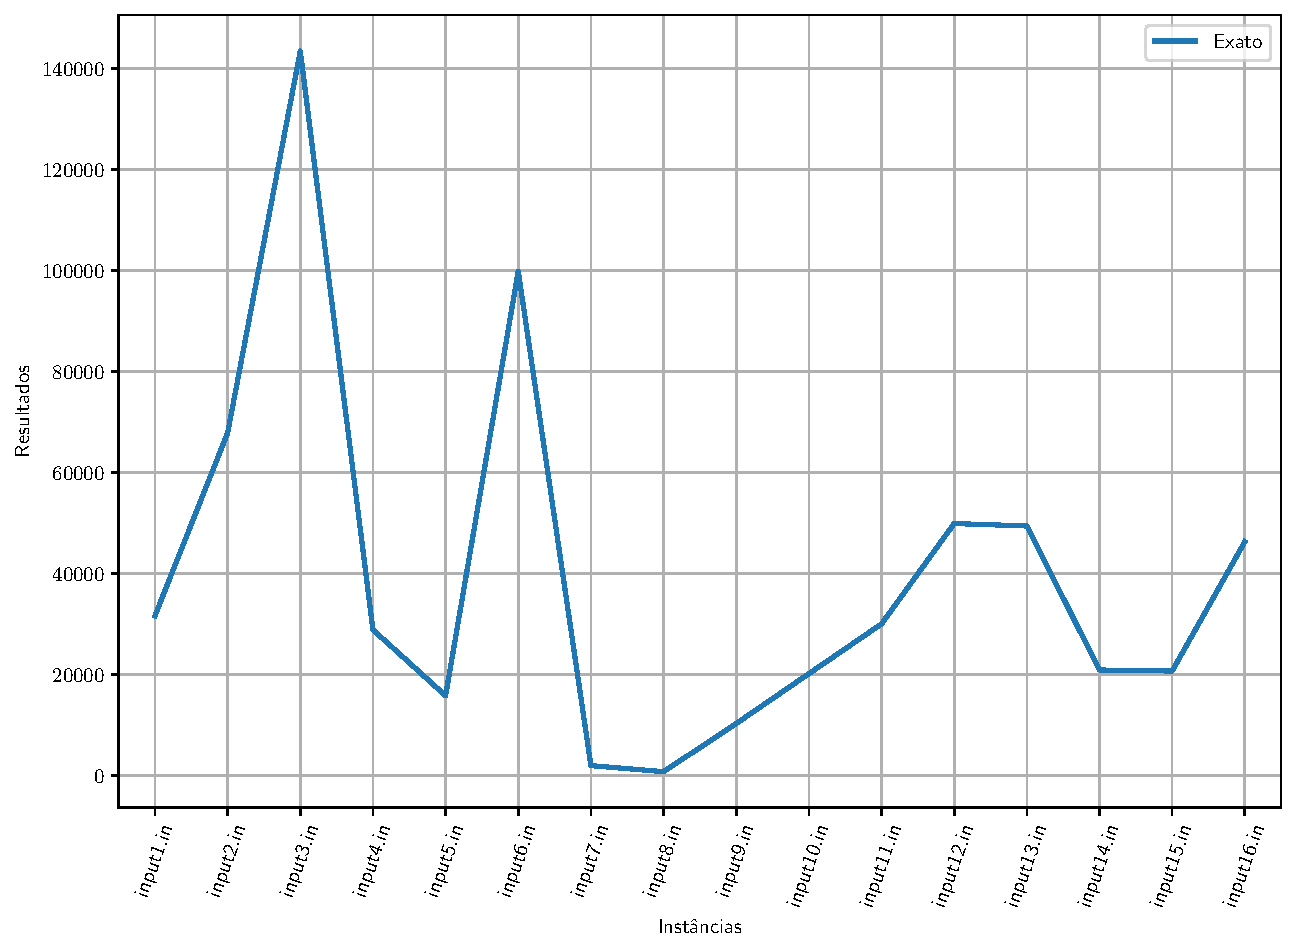
\includegraphics[width=1\linewidth]{../imgs/exact_results.pdf}
        \caption{Resultados exatos.}
        \label{exact_results}
    \end{minipage}%
    \begin{minipage}{0.5\textwidth}
        \centering
        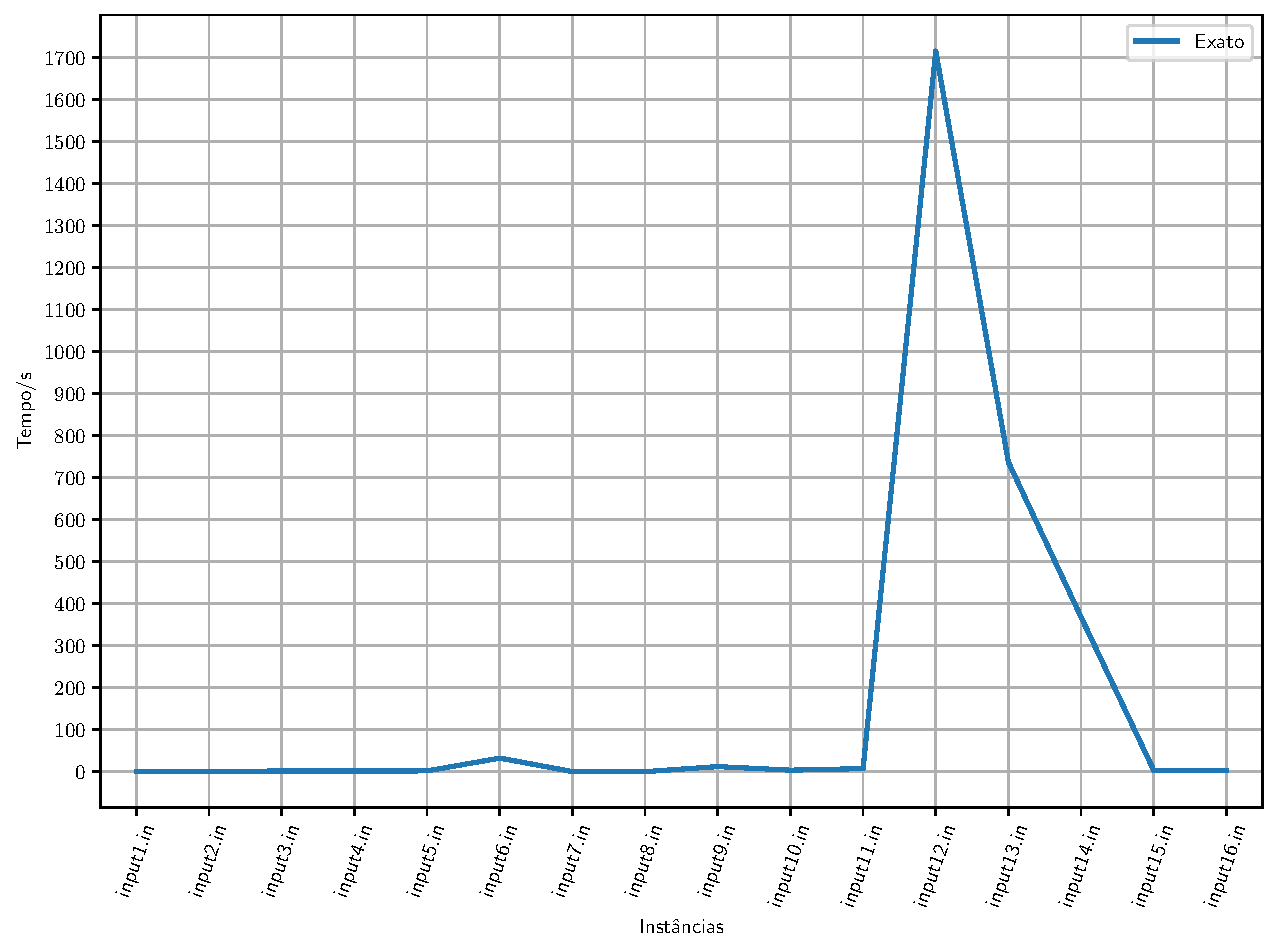
\includegraphics[width=1\linewidth]{../imgs/exact_time.pdf}
        \caption{Tempo para obtenção dos resultados.}
        \label{exact_time}
    \end{minipage}
\end{figure}

Como é possível observar na figura \ref{exact_time}, para algumas instâncias, o algoritmo retornou
o resultado ótimo instantaneamente, mas em contrapartida, para algumas instâncias o
tempo para obtenção do mesmo foi muito alto. Por exemplo, a instância \textit{"input12.in"},
demorou mais de \textit{1700 segundos}, ou seja, aproximadamente \textit{28 minutos}.

O objetivo então é tentar se aproximar o máximo possível desses resultados ou até mesmo chegar nesses,
mas em um tempo ideal.
% alcançar esses resultados ou chegar o mais próximo desses, em um tempo considerável.

\subsection{Heurísticas Gulosas}
A fim de melhorar o tempo na aquisição dos resultados, foram programadas três heurísticas gulosas.
Essas heurísticas foram nomeadas e desenvolvidas da seguinte forma:
\begin{itemize}
    \item \footnotesize{Crescente: O itens foram ordenados de acordo com seu respectivo peso, de forma crescente;} 
    \item \footnotesize{Decrescente: O itens foram ordenados de acordo com seu respectivo peso, de forma decrescente;}
    \item \footnotesize{Eficiente: Os itens foram ordenados de forma decrescente de acordo com a razão $\frac{valor}{peso}$.}
\end{itemize}

\begin{figure}[!htb]
    \centering
    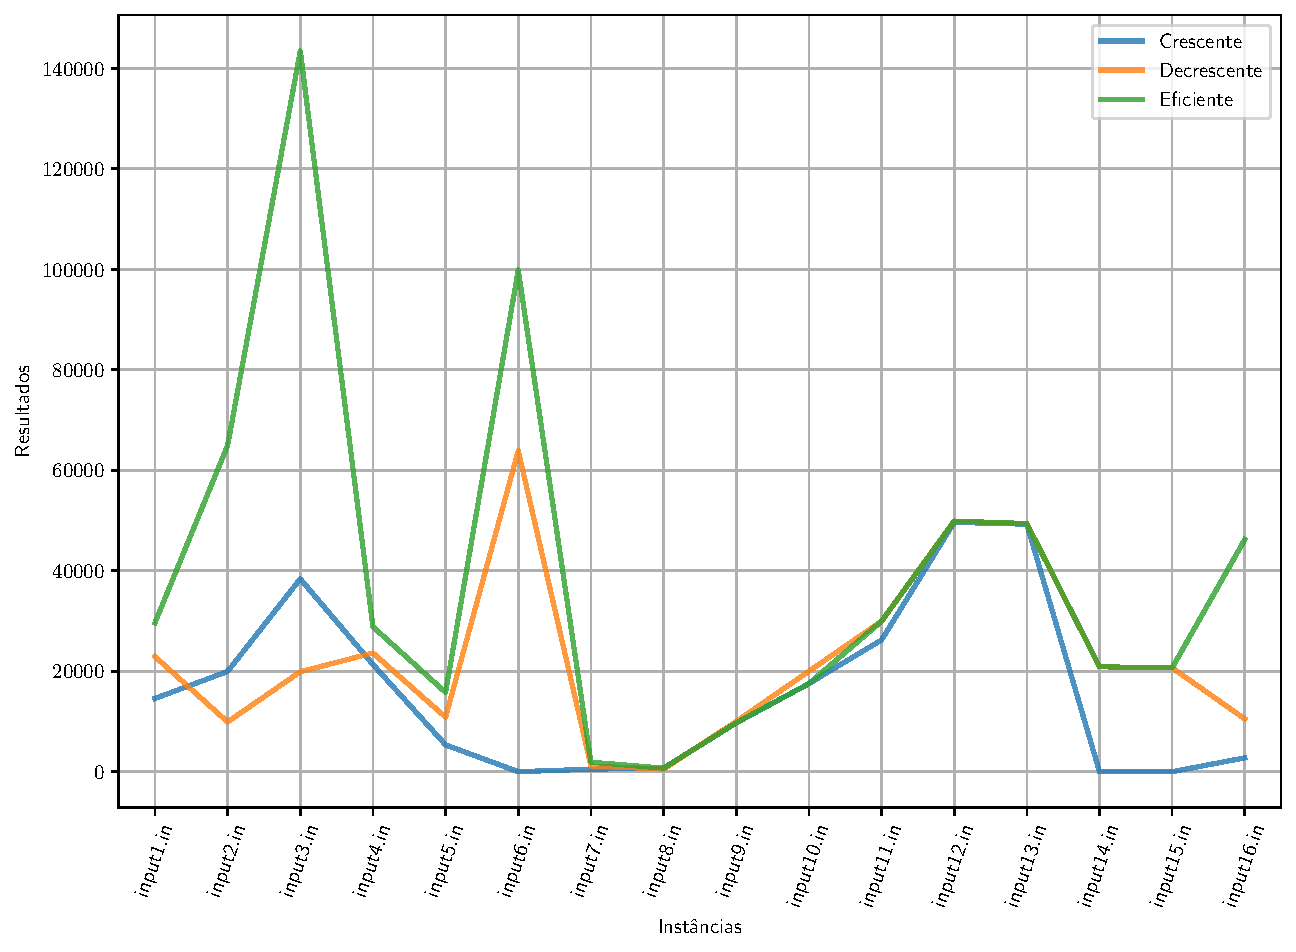
\includegraphics[width=0.7\linewidth]{../imgs/greedy_compare.pdf}
    \caption{Comparação entre resultados das Heurísticas Gulosas.}
    \label{greedy_compare}
\end{figure}

Como pode-se ver na figura \ref{greedy_compare}, existe uma grande discrepância entre os resultados obtidos 
de uma versão gulosa para outra e nesse caso, quanto maior o resultado obtido, melhor é o desempenho da heurística
quanto aos resultados ótimos, pois quanto maior esses resultados, mais próximo está da otimalidade.

Supostamente, das três heurísticas comparadas acima, a \textbf{Eficiente} se mostra a melhor, porém, com o intuito de provar
essa hipótese, foi realizado o cálculo do \textit{GAP} para cada instância e obtido a média desses valores, pois como
já foi calculado o resultado ótimo para cada instância, realizando este cálculo, é possível saber o quanto
o resultado desta heurística difere da otimalidade. Portanto, mais próximo de zero o GAP, melhor.

\begin{table}[htbp]
    \centering
    \resizebox{0.9\textwidth}{!}{
        \begin{minipage}{\textwidth}
            \centering
          \begin{tabular}{|c|c|}
                    \hline
                    \textbf{Heurísticas} & \textbf{GAP} \\
                    \hline
                    Crescente   &  49.594312 \\\hline
                    Decrescente &  27.347272 \\\hline
                    Eficiente   &   2.213083 \\\hline
            \end{tabular}  
          \caption{GAP médio - Heurísticas Gulosas}
          \label{tab:gap_greedy}
        \end{minipage}}
\end{table}

Logo, está provado que a heurística gulosa Eficiente é a melhor dentre as três apresentadas neste experimento.

\subsection{GRASP}
Para a obtenção dos resultados utilizando a metaheurístisca GRASP, a \textit{semente} para a geração
dos resultados randômicos foi definida com o valor de $42$. Ao definir um valor estático para a semente, 
os resultados que serão gerados
na fase de construção, partirão da mesma cadeia a cada iteração do GRASP. Ou seja, supondo que na primeira
iteração de uma janela qualquer o numero gerado foi $k$, então, na próxima iteração, após realizar a busca local,
a cadeia de números geradas randomicamente, partirá desse mesmo número $k$, portanto, é uma forma de evitar
que a cada iteração para uma mesma janela, o GRASP gere resultados totalmente aleatórios.

Com a intenção de escolher um bom valor para janela com o objetivo de obter de bons resultados locais,
foi realizado um experimento selecionando oito valores distintos para o tamanho da janela na escolha
de valores randômicos na fase de construção, esses valores estão no intervalo de $[2,9]$; foi escolhido assim,
pois se o tamanho da janela fosse $1$, este seria equivalente a uma heurística gulosa já visto acima, nomeada de 
\textbf{Eficiente} e caso o valor $10$ estivesse presente, iria acontecer um caso no número máximo de iterações
onde este seria equivalente ao \textbf{Algoritmo Aleatório}.

Além disso, também foi foram escolhidos quatro números diferentes
como critério de parada nas iterações do GRASP, isto é, o número máximo de iterações, os valores são
$10,100,1000$ e $10000$, ou seja, para cada valor distinto, o algoritmo só irá parar ao realizar este número de iterações.

Assim como afirmado acima na página \pageref{tab:gap_greedy}, quanto maior o resultado retornado por cada 
"variação" de uma heurística, melhor. Isto porque quanto maior for esse resultado, mais próximo ou igual 
está esse valor do resultado ótimo para cada instância.

Na figura \ref{all_grasp}, é possivel notar um comportamento interessante quanto aos resultados obtidos, isto porque,
para cada número máximo de iterações, os resultados se diferem um do outro quanto ao tamanho da janela, quando
o número de iterações é menor, ou seja, $10$ e $100$, para os outros valores, independente do tamanho da janela,
os resultados obtidos são praticamente os mesmos, por isso se observa um comportamento "constante".

\begin{figure}[h]
    \centering
    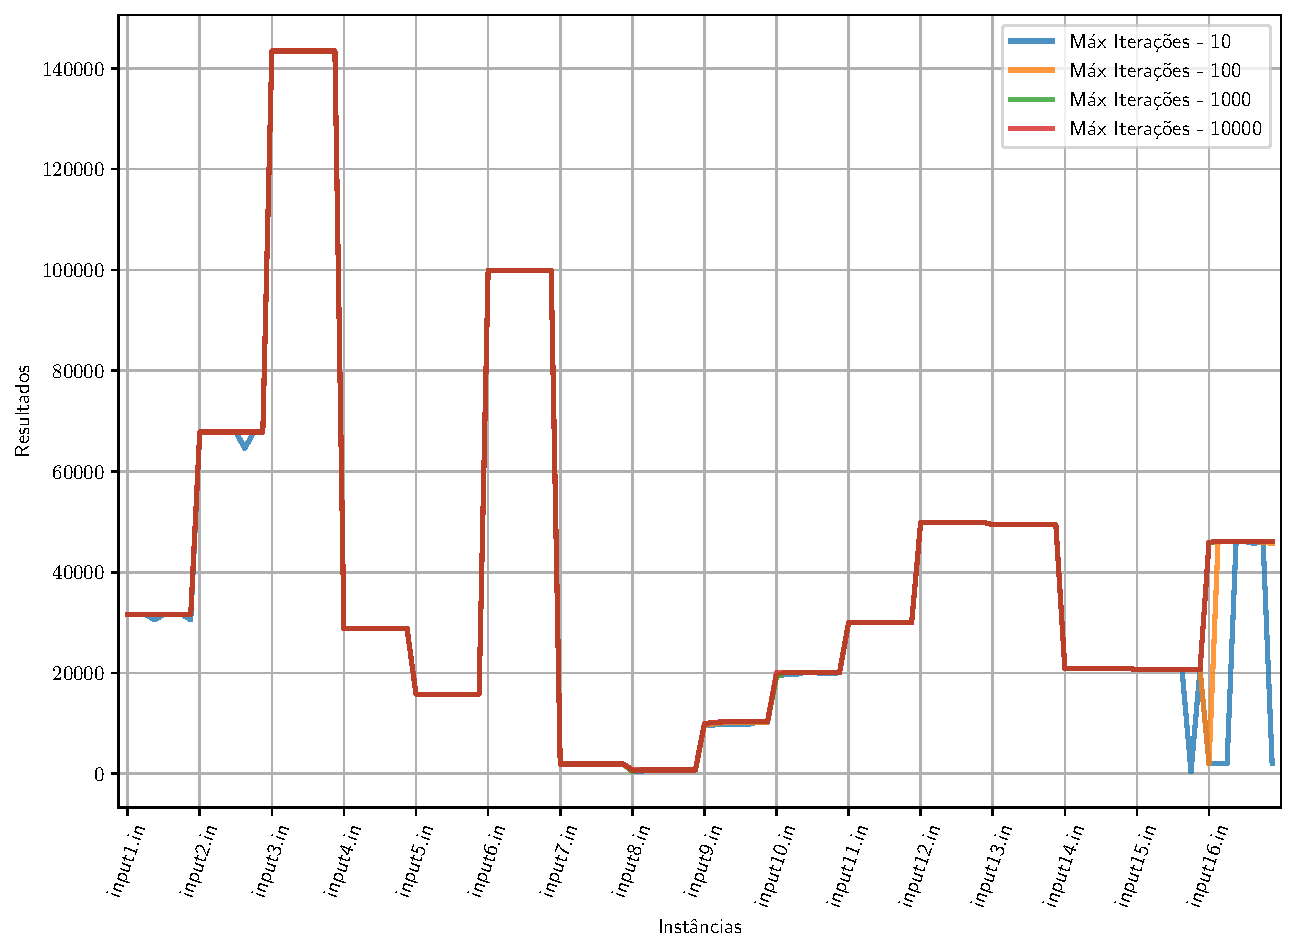
\includegraphics[width=0.7\linewidth]{../imgs/all_grasp.pdf}
    \caption{Resultados para as janelas e número de iterações específicos.}
    \label{all_grasp}
\end{figure}

A fim de escolher o melhor número de iterações para posteriormente analisar o melhor tamanho da janela
para estes experimentos, a figura \ref{gap_all_grasp} mostra o cálculo do GAP/Instância, considerando que para cada instância, existe varios 
tamanhos de uma janela, por isso é possivel notar alguns "picos" sobre o eixo num intervalo de uma mesma instância;
isso significa que para alguma janela deste mesmo número de iterações, o resultado divergiu mais da otimalidade.

\begin{figure}[h]
    \centering
    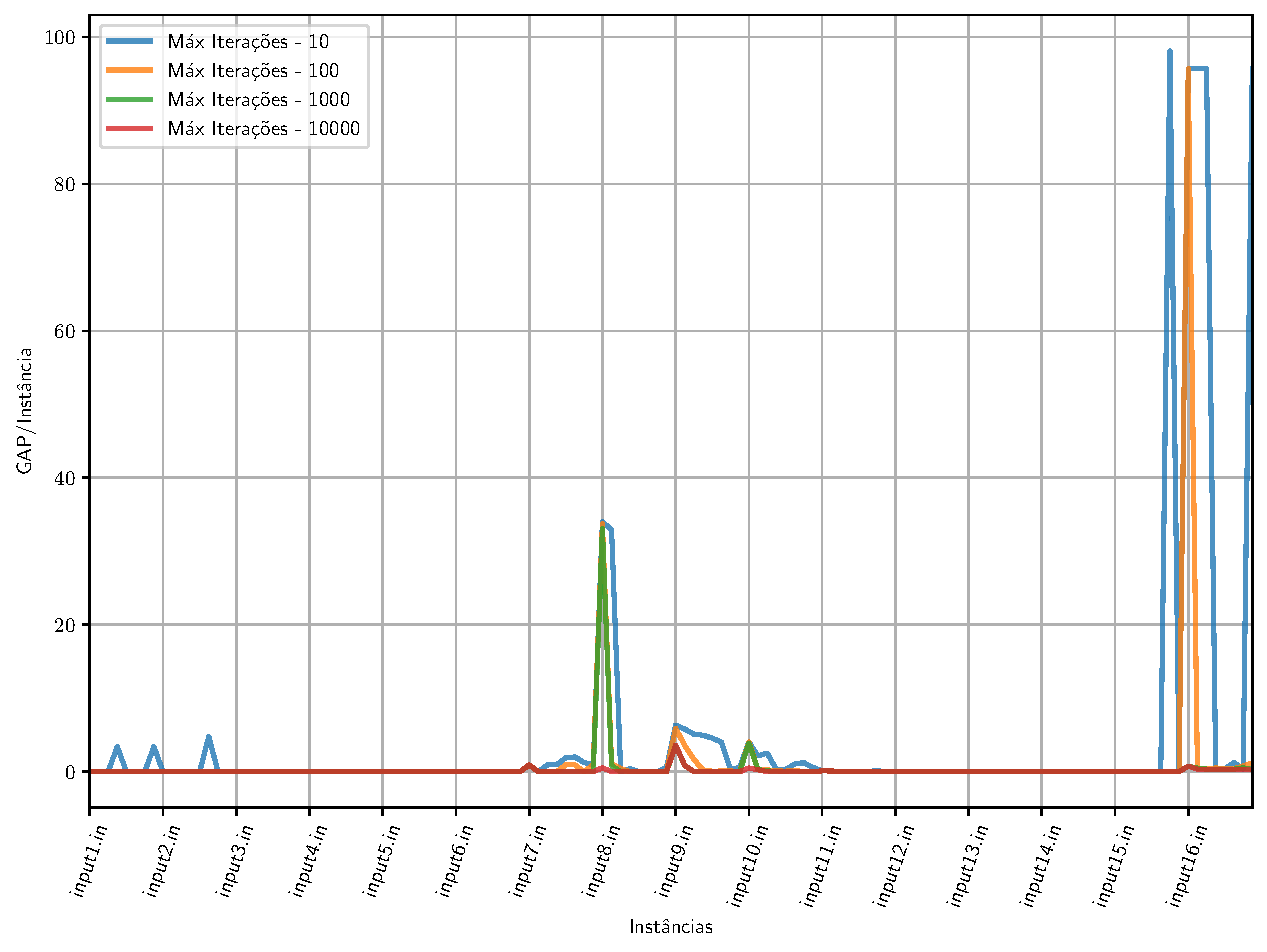
\includegraphics[width=0.7\linewidth]{../imgs/gap_all_grasp.pdf}
    \caption{GAP/Instância.}
    \label{gap_all_grasp}
\end{figure}

Supostamente, o número de iterações que mostra ser o melhor dentre os testados, é o de $10000$ iterações, a
tabela \ref{tab:gap_grasp}, apresenta o GAP médio para dos resultados para todas as janelas/iteração.

\begin{table}[htbp]
    \centering
    \resizebox{0.9\textwidth}{!}{
        \begin{minipage}{\textwidth}
            \centering
          \begin{tabular}{|c|c|}
                    \hline
                    \textbf{Heurísticas} & \textbf{GAP médio} \\
                    \hline
                    Máx Iterações - 10    &  4.811709 \\ \hline 
                    Máx Iterações - 100   &  1.217037 \\ \hline
                    Máx Iterações - 1000  &  0.370746 \\ \hline
                    Máx Iterações - 10000 &  0.080223 \\ \hline
            \end{tabular}  
          \caption{GAP médio para todas as janelas e iterações - GRASP}
          \label{tab:gap_grasp}
        \end{minipage}}
\end{table}

Portanto, pode-se afirmar que, de fato, para um número de iterações mais reduzido, o GAP é maior, pois
dependendo do tamanho da janela os resultados gerados podem se divergir muito e a tendência para um número
maior de iterações é que os vizinhos e resultados gerados, sejam cada vez mais próximos e melhores,
respectivamente.

A partir disso, foi selecionado somente os resultados gerados a partir de $10000$ iterações
e então foi desenvolvido uma lógica para escolher o melhor da janela dentre o intervalo $[2,9]$.

A lógica funciona da seguinte forma, para cada instância foi armazenado o índice das janelas que obteram
o maior valor dentre todas as janelas daquela instância. Por exemplo, para a instância \textit{"input1.in"},
todos as janelas obteram como resultado o mesmo valor, ou seja, o valor máximo era comum para todas as janelas
nessa instância, então foi armazenado o índice de todas as janelas na \textit{"input1.in"}.

Este procedimento foi realizado para todas as instâncias e ao final deste, o índice da janela que teve 
mais ocorrências de valores máximos foi escolhida como o melhor tamanho de janela para prosseguir com os testes. Se
ao final do procedimento, houver mais de um índice em comum para todas as instâncias, a de menor índice é selecionada.
Portanto, foi definido que o melhor tamanho de janela para essa quantidade de iterações foi a \textbf{Janela de tamanho 7.}

Então, a seguinte questão foi levantada: \textbf{"Será mesmo necessário realizar 10000 iterações para obter bons resultados?"}

Isto porque, esse número de iterações foi escolhido por causa do seu GAP médio, porém foi realizado o 
mesmo processo para escolher a melhor janela para os resultados que foram obtidos a partir de 1000 iterações,
que também obteve um bom GAP médio, mas ainda assim era inferior ao de 10000 iterações.

Surpreendentemente, a janela que obteve os melhores resultados tambem foi a janela 7, nesse caso, foi calculado
o GAP médio somente para esta janela, nas duas versões em questão.

\begin{table}[htbp]
    \centering
    \resizebox{0.8\textwidth}{!}{
        \begin{minipage}{\textwidth}
            \centering
          \begin{tabular}{|c|c|}
                    \hline
                    \textbf{Versões - GRASP} & \textbf{GAP médio} \\
                    \hline
                    GRASP 1000 it.  &  0.022221 \\ \hline
                    GRASP 10000 it. &  0.021815 \\ \hline
            \end{tabular}  
          \caption{GAP médio - GRASP}
          \label{tab:gap_grasp}
        \end{minipage}}
\end{table}

Ainda assim, mesmo para essa janela específica, o GAP da versão de 10000 iterações é pouca coisa menor que o de 1000 iterações.
Entretanto, foi realizado uma análise do tempo de execução para essas duas versões do GRASP em questão, para levar
em consideração se vale pena sacrificar um centésimo de um resultado mais próximo da otimalidade, para 
considerar o que demanda menos custo computacional.

% Ou seja, e possivel ver que o gap para 10000 iteracoes é menor do que para 1000 iteracoes, logo, poderia afirmar
% que este é o melhor a ser usado dentro todos os valores testados?

% Para isso foi realizado uma analise de tempo, ou seja, quanto tempo levou para obter esses resultados, considerando
% que a disparidade destes dois gap's é bem pequena, pode-ser que seja melhor utilizar as 1000 iteracoes em vez
% das 10000.

% Ou seja, pode ser que seja melhor utilizar os resultados obtidos pela versão ate 1000 iterações, para a mesma janela.
% Pode-se notar na figura \ref{grasp_compare_1kvs10k} que isso se comprova, afinal, são 9000 iterações a menos.

\begin{figure}[h]
    \centering
    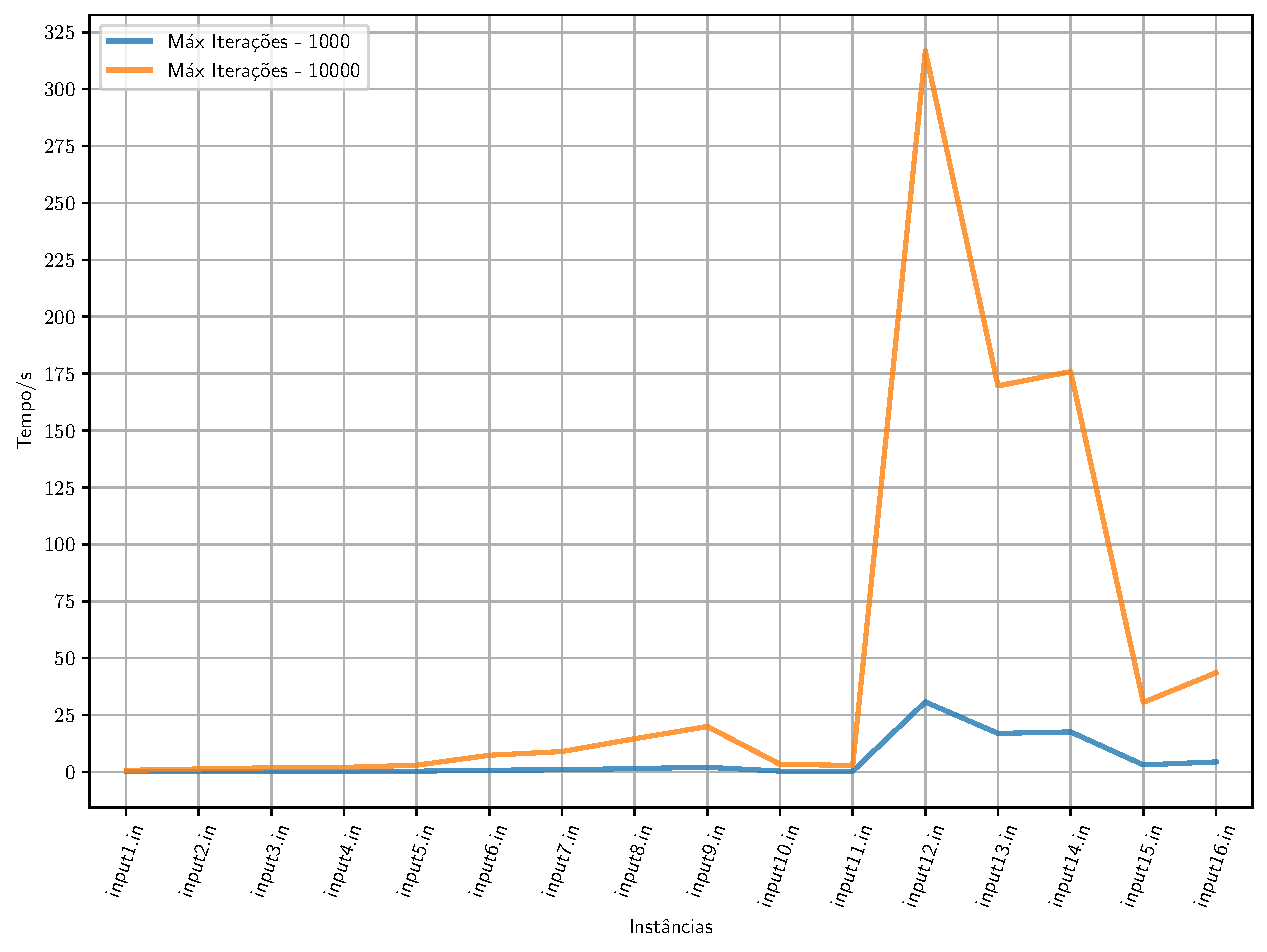
\includegraphics[width=0.7\linewidth]{../imgs/grasp_compare_1kvs10k.pdf}
    \caption{Comparação entre resultados das Heurísticas Gulosas.}
    \label{grasp_compare_1kvs10k}
\end{figure}

Pode-se observar na figura \ref{grasp_compare_1kvs10k} e na tabela \ref{tab:sum_time_grasp} 
a diferença para obtenção de cada resultado por instância e o tempo total para cada variação do GRASP, respectivamente.
É possivel afirmar que a disparidade 
de tempo na obtenção dos resultados existe e é considerável para uma diferença tão pequena no GAP médio, ou seja, é possivel
afirmar também que após 1000 iterações pouco alterou os resultados obtidos em busca de uma 
melhor solução local. 

\begin{table}[htbp]
    \centering
    \resizebox{0.8\textwidth}{!}{
        \begin{minipage}{\textwidth}
            \centering
            \begin{tabular}{|c|c|c|}
                    \hline
                    \textbf{Versões - GRASP} & \textbf{Tempo/s} & \textbf{Speed-up} \\
                    \hline
                    Máx Iterações - 10000 & 801.770529 & - \\ \hline
                    Máx Iterações - 1000  &   79.166350 & 10.1276 \\ \hline
                       
            \end{tabular}  
          \caption{Somatório do tempo para obtenção dos resultados.}
          \label{tab:sum_time_grasp}
        \end{minipage}}
\end{table}

A tabela \ref{tab:sum_time_grasp} também mostra o \textbf{Speedup} obtido da versão de 10000 iterações para
a versão de 1000 iterações, e como pode-se ver, a versão de 1000 iterações é 10 vezes mais rápida que a versão
de 10000 iterações, o que em recurso computacional é muito relevante.
Portanto, foi definido que a melhor versão do GRASP dentre as testadas, em relação a custo/benefício,
é a versão de 1000 iterações com a janela de tamanho 7.



\section{Conclusão}

A figura \ref{final_compare} mostra a comparação final entre a melhor heurística gulosa e a melhor variação do GRASP
dentre as testadas, com os resultados exatos. A figura \ref{time_final_cmp} apresenta tempo em que cada
algoritmo obteve tal resultado.

\begin{figure}[!htb]
    \centering
    \begin{minipage}{0.5\textwidth}
        \centering
        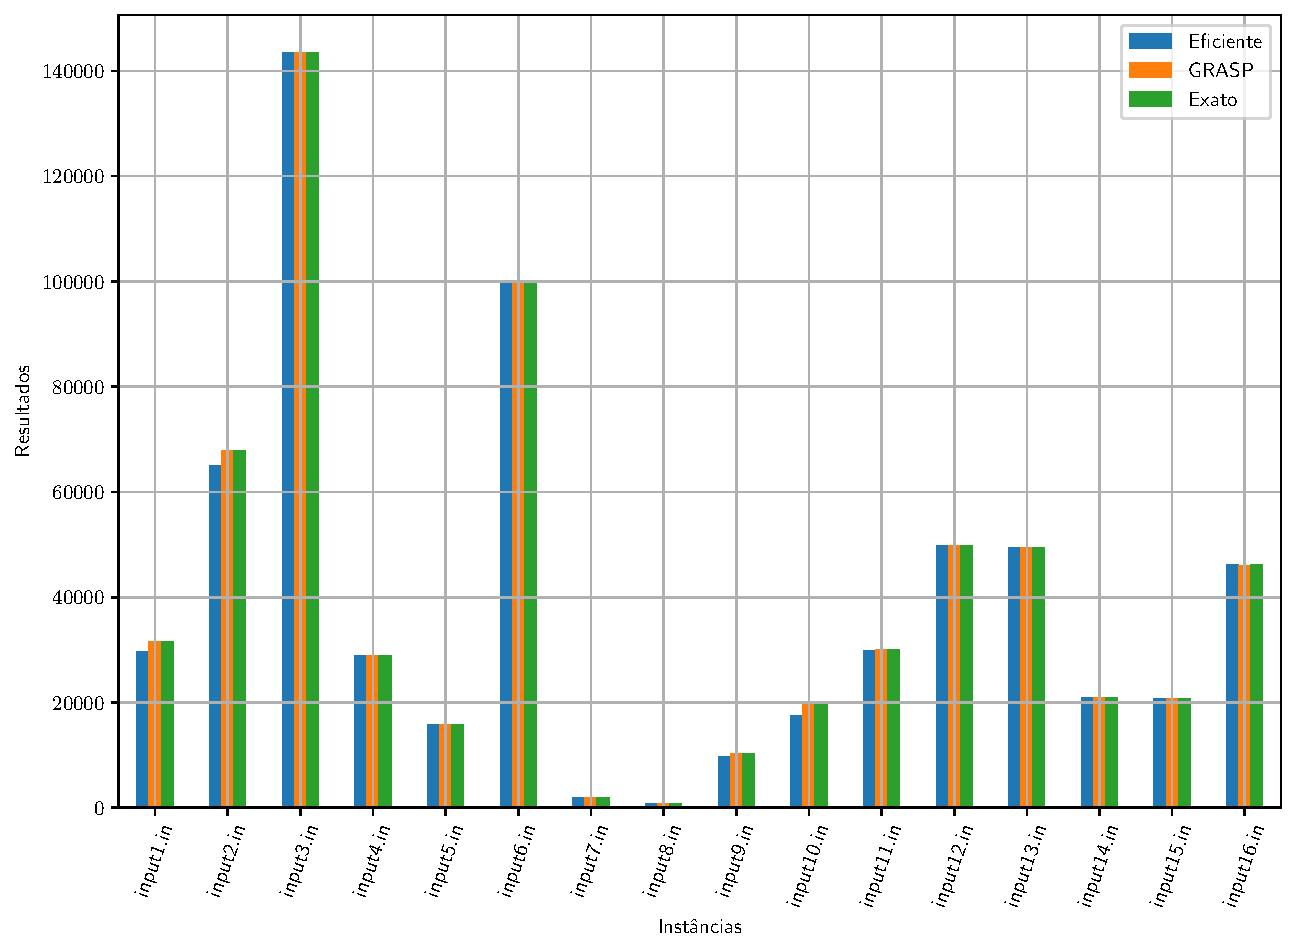
\includegraphics[width=\linewidth]{../imgs/final_compare.pdf}
        \caption{Comparação entre os resultados finais.}
        \label{final_compare}
    \end{minipage}%
    \begin{minipage}{0.5\textwidth}
        \centering
        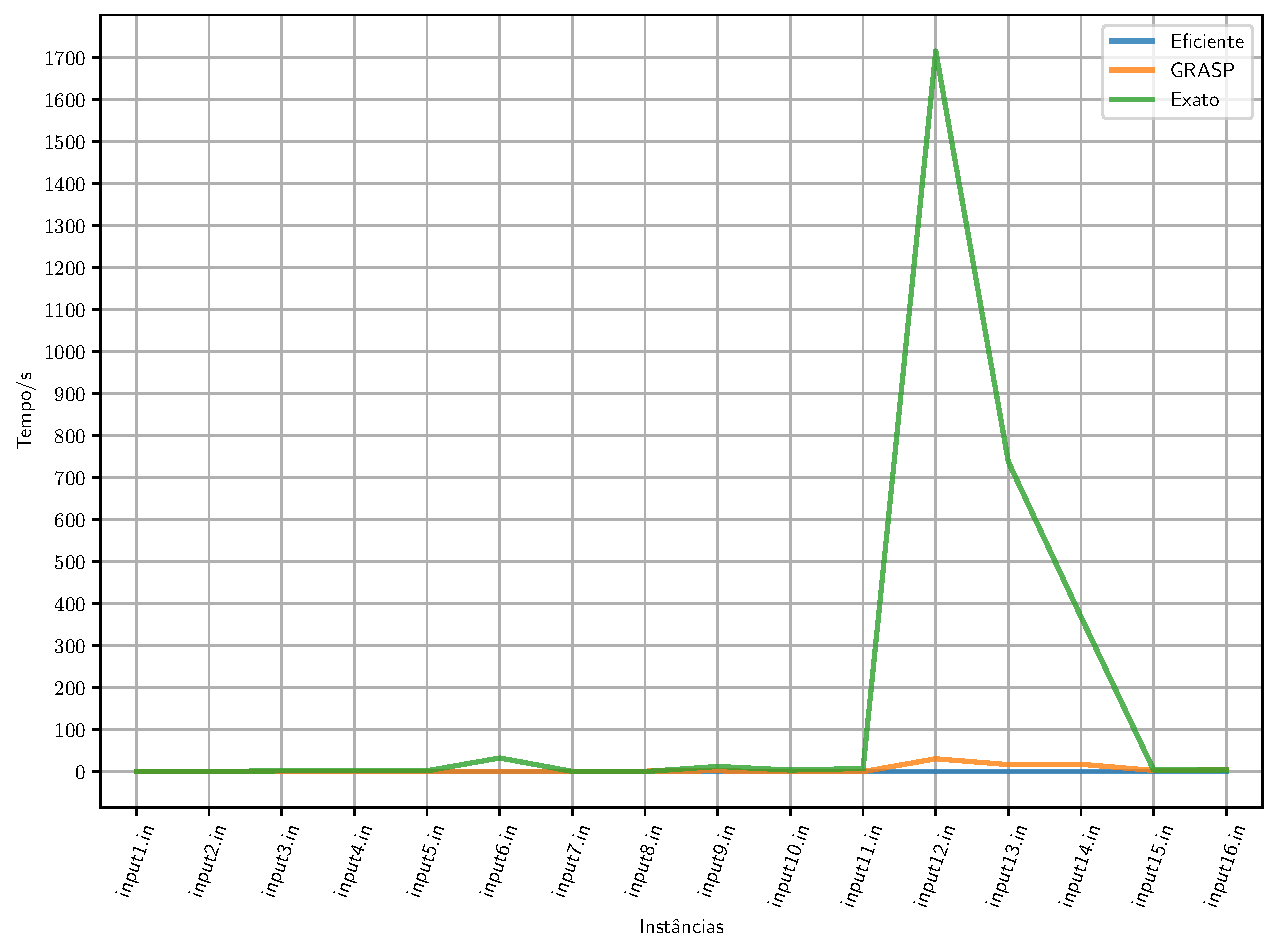
\includegraphics[width=1\linewidth]{../imgs/time_final_cmp.pdf}
        \caption{Comparação de tempo para obtenção dos resultados entre os algoritmos.}
        \label{time_final_cmp}
    \end{minipage}
\end{figure}

A tabela \ref{tab:cmp_greedy_grasp} mostra o tempo total em segundos, Speedup e o GAP para cada heurística programada.
Como o algoritmo Exato é utilizado como base de comparação, o mesmo não possui Speedup e nem GAP.
\begin{table}[htbp]
    \centering
    \resizebox{0.8\textwidth}{!}{
        \begin{minipage}{\textwidth}
            \centering
            \begin{tabular}{|c|c|c|c|}
                    \hline
                    \textbf{Algoritmos} & \textbf{Tempo/s} & \textbf{Speedup} &\textbf{GAP médio} \\
                    \hline
                    Exato     & 2893.456222 & -          & - \\ \hline
                    GRASP     & 79.166350   & 36.5490    & 0.022221 \\ \hline
                    Eficiente & 0.029479    & 98153.1334 & 2.213083\\ \hline
            \end{tabular}  
          \caption{GAP entre as melhores Heurísticas testadas.}
          \label{tab:cmp_greedy_grasp}
        \end{minipage}}
\end{table}

Pode-se concluir que os resultados alcançados foram satisfatórios. As heurísticas não alcançaram a otimalidade
, bem como visto na página \ref{nphard}, porém, foram bons resultados em relação a tempo/instância. É importante
notar que, as instâncias disponibilizadas não são tão grandes e mesmo assim, a obtenção do resultado ótimo
demandou bastante tempo, logo, é inviável utilizar um algoritmo exato para a obtenção de tal resultado num cenário
onde as instâncias ultrapassam 100000 itens por exemplo.

\bibliography{References}{}
\bibliographystyle{plain}

\end{document}